\documentclass{beamer}
\usetheme{Szeged}
\usecolortheme{seahorse}
\usepackage{hyperref}
\usepackage[utf8]{inputenc}

\title{Model Thinker Topics}
\author{Tristan Goodell, Nikki Weatherington, Jacob Holmes}
\institute[]{Arkansas School for Mathematics, Sciences, and the Arts}
\date{4 September 2019}

\begin{document}

\maketitle

\begin{frame}{John Conway's Game of Life}

    \begin{itemize}
        \item The Game of Life is a cell replication simulation created by John Conway. Depending on the initial placement of cells, patterns may be created.
        \item The Game of Life abides by the following mathematical rules:
        \begin{itemize}
            \item For a space that is populated: 
            \begin{itemize}
                \item Each cell with one or no neighbors dies, as if by solitude.$^1$ 
                \item Each cell with four or more neighbors dies, as if by overpopulation.$^1$  
                \item Each cell with two or three neighbors survives.$^1$  
            \end{itemize}
            \item For a space that is 'empty' or 'unpopulated':
            \begin{itemize}
                \item Each cell with three neighbors becomes populated.$^1$  
            \end{itemize}
        \end{itemize}
        \item Simulation can be found \bf \href{https://bitstorm.org/gameoflife/}{here}. 
    \end{itemize}
    \footnote{https://bitstorm.org/gameoflife/}
\end{frame}

\begin{frame}{The Simpson's Paradox}
    \begin{itemize}
        \item The Simpson's Paradox happens when the average of each of multiple groups of data is higher than the corresponding average of other groups of data, but the overall averages between the sets of the different groups shows a different trend.
        \item The formal definition is shown by the following formula.
        \begin{itemize}
            \item 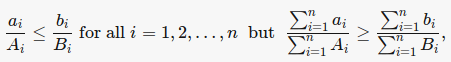
\includegraphics[scale=.4]{simpsonsparadox.png}
        \end{itemize}
        \item This paradox occurs when the groups that are compared initially are different sizes.
        \begin{itemize}
            \item An exaggerated example is
            \begin{center}
                \begin{tabular}{||c c c||} 
                    \hline
                    Day & You & Friend \\ [0.5ex] 
                    \hline\hline
                    1 & $\frac{998}{1000}$ & $\frac{2}{2}$ \\ 
                    \hline
                    2 & $\frac{0}{2}$ & $\frac{2}{1000}$ \\
                    \hline
                    Overall & $\frac{998}{1000}$ & $\frac{4}{1000}$ \\
                    \hline
                \end{tabular}
            \end{center}
        \end{itemize}
    \end{itemize}
\end{frame}

\end{document}
